Στο συγκεκριμένο κεφάλαιο παρουσιάζεται το θεωρητικό υπόβαθρο πάνω στο οποίο βασίστηκε η μελέτη της πτυχιακής εργασίας που ακολουθεί.
Ειδικότερα η απαραίτητη θεωρία των μη-γραμμικών δυναμικών συστημάτων, τα εργαλεία που χρησημοποιήθηκαν για την μελέτη των συστημάτων, όπως και τα φαινόμενα που παρατηρήθηκαν κατα την διάρκεια της μελέτης.

\section{Δυναμικά συστήματα}

	
Αν θεωρήσουμε ένα Ν-διάστατο χώρο εξαρτημένων μεταβλητών $x_k(t), k =1, 2, ...., N$, που έχουν ώς μόνη ανεξάρτητη μεταβλητή τους το χρόνο  $t$ και αποτελούν συνιστώσες του διανύσματος :

\begin{equation}	
	x (t)= \bigl( x_1(t) , x_2(t), .... , x_N(t) \bigl) ,\quad t \in I= (α,β)
	\label{m:g1}
\end{equation}

όταν ο χρόνος είναι \textbf{συνεχής} στο διάστημα \textbf{I} (οι μεταβλητές θεωρούνται πραγματικές) ή ενός διανύσματος :

\begin{equation}	
x_n = x(t_n)= \bigl( x_{1,n}, x_{2,n}, .... , x_{N,n} \bigl) , \quad x(k_n)= x_k(t_n)
\label{m:g2}
\end{equation}

όταν ο χρόνος παίρνει \textbf{διακριτές} τιμές $t_n$ ($n$ ακέραιος).
Η εξέλιξη στο χρόνο των διανυσμάτων αυτών, δίνεται απο ένα σσυτημα 
\emph{διαφορικών εξισώσεων} πρώτης τάξης αν το $t$ είναι συνεχές :
\begin{equation}
	\frac{d\textbf{x}}{dt} = \textbf{x} = \textbf{f}(\textbf{x},t)  \quad  \text{ή} \quad  
		  x_k = f_k (\textbf{x},t), \quad k=1,2, .... , N ,
	\label{m:g3}
\end{equation}

ή ένα σύστημα εξισώσεψν διαφορών

\begin{equation}	
	x_{n+1} = \textbf{g}(\textbf{x}_n), \quad \text{ή}  \quad x_{k,n+1}= g_k(\textbf{x}_n), \quad k=1,2, .... , N
	\label{m:g4}
\end{equation}

αν $t$ διακριτό και ορίζεται ως το δυναμικό σύστημα που περιγράφει το φυσικό φαινόμενο που μας ενδιαφέρει. Οι διανυσματικές συναρτήσεις \textbf{f} και \textbf{g} αποτελούν την "μαθητικοποίηση"
του φαινομένου και φυσικά διαφέρουν ανάλογα με τους φυσικούς νόμους που διέπου κάθε φαινόμενο. Ο Ευκλείδιος χώρος $ \mathbb{R} ^Ν$ στον οποίον εξελίσσονται τα διανύσματa $\textbf{x}(t)$ και $\textbf{x}(n)$ λέγεται \textbf{χώρος φάσεων του συστήματος}.\cite{b1}

\newpage

Συμβολικά, λοιπόν, μπορούμε να ορίσουμε ένα δυναμικό σύστημα ως μια \textbf{ροή} (ή απεικόνιση)  $φ(x,t)$  στο χώρο φάσεων:
\begin{equation}
 φ: R\times E \to E ,
\end{equation}
η οποία μεταφέρει (ή απεικονίζει) ένα σημείο $\textbf{x}=(x_1,x_2,....,x_n)$ , το οποίο αντιστοιχεί στη θέση του
συστήματος τη χρονική στιγμή $t$, σε ένα
σημείο $\textbf{x'}=(x_1,x_2,....,x_n)$, το οποίο αντιστοιχεί στη θέση του συστήματος τη χρονική στιγμή $t'$,

\begin{equation}
\textbf{x}=φ(x,t)
\end{equation}

Μια ροή έχει τις ιδιότητες:

\begin{gather}
φ(\textbf{x},0)=\textbf{x} \\
φ(φ(\textbf{x},t_1),t_2)=φ(\textbf{x},t_1+t_2)
\end{gather}
Μπορούμε να ορίσουμε τη θέση $x_0 = (x_10, x_20,...., x_{n0})$ σε μια χρονική στιγμή $t_0$ ως την αρχική θέση του
συστήματος. Αρχική θέση για το σύστημα μπορεί να αποτελεί κάθε σημείο του χώρου των φάσεων και η ροή $φ(x,t)$ του δυναμικού συστήματος μπορεί να εφαρμοστεί σε οποιαδήποτε αρχική θέση του συστήματος. Εν γένει, η εξέλιξη του συστήματος που αντιστοιχεί σε διαφορετική αρχική θέση είναι επίσης διαφορετική. Αν ο κανόνας εξέλιξης που εκφράζεται με την ροή δεν εμπλέκει «τυχαιότητα» τότε το σύστημα ονομάζεται \textbf{αιτιοκρατικό} (deterministic). Ένα αιτιοκρατικό σύστημα δίνει πάντα την ίδια εξέλιξη για μια δοθείσα αρχική θέση. Αν η ροή συμπεριλαμβάνει κάποιον βαθμό τυχαιότητας με τον ορισμό πιθανοτήτων στον κανόνα της εξέλιξης τότε το σύστημα ονομάζεται \textbf{στοχαστικό} (stochastic). 

Αν η ροή $φ(x,t)$ ενός αιτιοκρατικού συστήματος δεν εξαρτάται ρητά από το χρόνο $t$ τότε το σύστημα ονομάζεται αυτόνομο. Σε ένα τέτοιο σύστημα, η εξέλιξη του συστήματος είναι ανεξάρτητη από την αρχική
χρονική στιγμή. Αντίθετα, σε ένα μη-αυτόνομο σύστημα, αν το σύστημα βρεθεί σε ένα σημείο $x \in E$, η εξέλιξή του στο χρόνο εξαρτάται και από την χρονική στιγμή t στην οποία βρίσκεται στο \textbf{x}.

Αν και στη φύση ο χρόνος $t$ αποτελεί μια συνεχή μεταβλητή, σε ένα δυναμικό σύστημα ο χρόνος μπορεί να είναι συνεχής ή διακριτός.\cite{b2}



\subsection{Συνεχές δυναμικό σύστημα}
 
Στην πρώτη περίπτωση ο χρόνος μπορεί να πάρει μια οποιαδήποτε πραγματική τιμή και το δυναμικό σύστημα ονομάζεται \textbf{συνεχές}.\cite{b2}

\subsection{Διακριτό δυναμικό σύστημα}
Αν όμως η εξέλιξη του συστήματος περιγράφεται σε χρονικά βήματα ανά $ΔT$ τότε ο χρόνος παίρνει τις διακριτές τιμές $t_k = t_0 + kΔt$ και το σύστημα ονομάζεται \textbf{διακριτό} (discrete). 
Για ένα διακριτό σύστημα μια χρονική στιγμή $t \in(t_k,t_{k+1}) $ δεν έχει νόημα.\cite{b2}



Στη συγκεκριμένη εργασία όλα τα συστήματα που μελετήθηκαν ανήκουν στην κατηγορία των διακριτών, μη - γραμμικών συστημάτων

\clearpage

\section{Χαοτική συστήματα}

Τα χαοτικά συστήματα αποτελούν μια ξεχωριστή αυτοδύναμη κατηγορία δυναμικών συστημάτων, που μπορεί να τοποθετηθεί μεταξύ ντετερμινιστικών και στοχαστικών συστημάτων. Αν και φαίνονται στοχαστικά όταν παρατηρούνται, παρ’ όλα αυτά περιγράφονται μαθηματικά από μη γραμμικές διαφορικές εξισώσεις (ροές) ή από μη
γραμμικές εξισώσεις διαφορών (απεικονίσεις) και ανήκουν στην κατηγορία των μη γραμμικών καταναλισκόντων συστημάτων. Η τροχιά τους για ένα σύνολο αρχικών συνθηκών που αποτελούν την βάση ελκυσμού, περιορίζεται σε ένα υπόχωρο του χώρου φάσεων που στην προκειμένη περίπτωση επειδή εμφανίζει πρωτότυπες (παράξενες) ιδιότητες λέγεται παράξενος ελκυστής. Αν και ο χώρος που εξελίσσεται η τροχιά είναι περιορισμένος, αυτή δεν διέρχεται ποτέ από το αυτό σημείο δύο φορές, δηλαδή δεν κόβει τον εαυτό της, έχει άπειρο μήκος, είναι απεριοδική και τούτο φαίνεται καθαρά στο φάσμα ισχύος μια μεταβλητής του συστήματος που είναι συνεχές. Επίσης φαίνεται να περιφέρεται τυχαία, δηλαδή οι μελλοντικές θέσεις της να μην σχετίζονται με τις παρελθούσες, για αυτό και ο συντελεστής αυτοσυσχέτισης μια μεταβλητής ενός χαοτικού συστήματος μηδενίζεται
σε σχετικά μικρό χρονικό διάστημα.\cite{b3}




\clearpage

\section{Χαοτικά χαρακτηριστηκά}
Το κύριο χαρακτηριστικό των χαοτικών συστημάτων, είναι η
ευαίσθητη εξάρτηση από τις αρχικές συνθήκες. Δηλαδή, αν δοθούν δύο τυχαίες διαφορετικές αρχικές συνθήκες $x_1(0)$ και $x_2(0) = x_1(0) + Δt(0) $, η μια κοντά στην άλλη, οι τροχιές που προκύπτουν αποκλίνουν μέχρινα γίνουν ασυσχέτιστες.

 
\section{Εργαλεία μελέτης χαοτικών συστημάτων}
Τα βασικά εργαλεία που χρησιμοποιήθηκαν στην μελέτη της εργασίας αναλύονται παρακάτω:

\subsection{Διάγραμμα Διακλάδωσης}

Tα διαγράμματα διακλάδωσης χρησιμοποιούνται κυρίως για την ποιοτική μελέτη της ροής ενός χαοτικού συστήματος αλλάζοντας μία παράμετρο \emph{k}. Συγκεκριμένα σημεία ισορροπίας μπορούνε να δημιουργηθούν ή να καταστραφούν ή να αλλάξει η ευστάθεια τους. Τέτοιες ποιοτηκές μεταβολές σε ένα σύστημα της ονομάζουμε \textbf{διακλαδώσεις} και οι τιμές των παραμέτρων κατα τις οποίες εμφανίζονται αυτές οι αλλαγές ονομάζονται \textbf{σημεία διακλάδωσης}. Στα διαγράμματα διακλάδωσης,παρατηρούμε τόσο χαοτικές όσο και περιοδικές περιοχές, ενώ στην περίπτωση που εξετάζουμε ένα χαοτικό σύστημα , παρατηρούνται φαινόμενα όπως ο \emph{διπλασιασμός περιόδου} ,η \emph{υστέρηση}, \emph{συνύπαρξη ελκυστών},η \emph{αντιμονοτονικότητα} και η \emph{κρίση ελκυστών} τα οποία θα αναλυθούν στην επόμενη παράγραφο.\cite{b4}

\subsection{Εκθέτης Lyapunov}
Ο εκθέτης Lyapunov μιας απεικόνισης αποτελεί ένα μέτρος της ευαισθησίας της εξάρτησης από τις αρχικές συνθήκες, η οποία είναι χαρακτηριστική της χαοτικής συμπεριφοράς ενός συστήματος. Ο εκθέτης (συμβολίζεται με \emph{λ}), μπορεί να υπολογιστεί για μία μονοδιάστατη απεικόνιση. Αν ένα σύστημα μπορεί να εξελιχθεί απο δύο διαφορετικές καταστάσεις , $x$ και $ x + ε_0$ τότε μετά απο $n$ επαναλήψεις η απόκλιση των δύο καταστάσεων δίνεται από τη σχέση

\begin{equation}
	ε(n) = ε_02^λn
\end{equation}

όπου ο εκθέτης Lyapunov λ δίνει τη μέση τιμή του ρυθμού απόκλισης. Αν ο λ είναι αρνητικός, τότε η εξέλιξη του συστήματος δεν οδηγεί σε χαοτική συμπεριφορά γιατί οι τροχιές συγκλίνουν. Αν ο λ είναι θετικός, τότε οι γειτονικές τροχιές αποκλίνουν, οπότε η εξέλιξη του συστήματος είναι ευαίσθητη στις αρχικές συνθήκες που είναι το κύριο χαρακτηριστηκό του χάους.\cite{b5}
\clearpage

\section{Φαινόμενα χαοτικών συστημάτων}
Τα φαινόμενα που θα αναλυθουν παρακάτω παρατηρήθηκαν στα συστήματα που μελετήθηκαν στα επόμενα κεφάλαια.

\subsection{Διπλασιασμός περιόδου}

Αυτό το φαινόμενο παρατηρείται σε χαοτικά συστήματα όπως η λογιστική απεικόνιση. Ουσιαστικά οι διακλαδώσεις σε ένα διάγραμμα όπως το \ref{th:g1} όσο αυξάνεται η παράμετρος \emph{k} διπλασιάζονται απο περίοδο-1 σε περίοδο-2 μέχρι που για συγκεκριμένο \emph{k} το σύστημα εισέρχεται σε χάος.


\begin{figure}[ht]
	\centering
	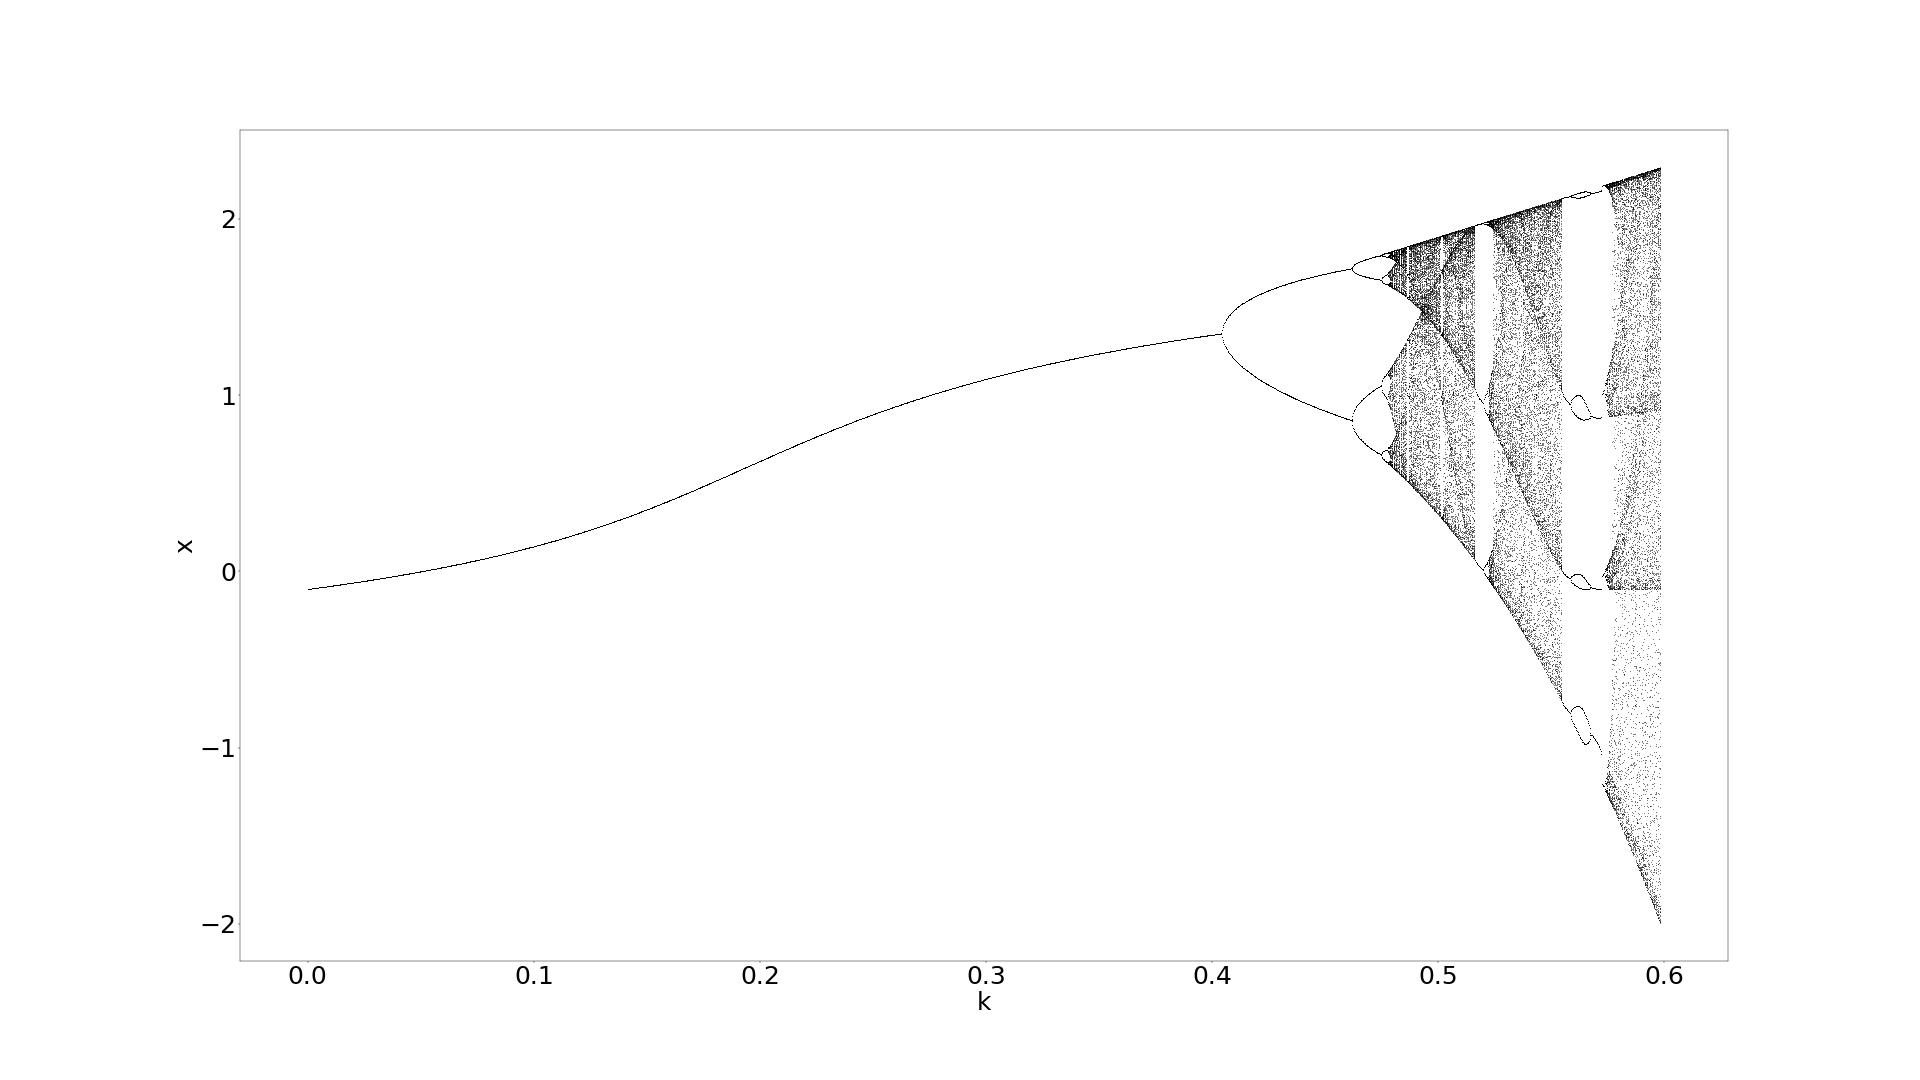
\includegraphics[width=1\linewidth]{LateX images/graphs/g1}
	\caption{ Διάγραμμα διακλάδωσης.}
	\label{th:g1}	
\end{figure}

\subsection{Υστέρηση}
Όταν μεταξύ των ορίων διαφόρων περιοδικών περιοχών υπάρχει ασυνέχεια, τότε αυτό ονομάζεται φαινόμενο υστέρησης.

\subsection{Κρίση ελκυστών}

Όταν παρατηρούμε μία απότομη ασυνεχή μεταβολή σε ένα χαοτικό ελκυστή
ενώ μεταβάλλεται μία παράμετρος του συστήματος,το ονομάζουμε κρίση ελκυστών. 
Οι ασυνεχείς μεταβολές είναι τυπικά τριών τύπων
\begin{enumerate}
\item Ένας χαοτικός ελκυστής καταστρέφεται καθώς η παράμετρος περνά από μια κρίσιμη τιμή.Το είδος αυτής της κρίσης ονομάζεται συνοριακή κρίση (boundary crisis).
\item Το μέγεθος του χαοτικού ελκυστή στο χώρο των φάσεων αυξάνεται ξαφνικά καθώς η παράμετρος περνά από την κρίσιμη τιμή της παραμέτρου. Το είδος αυτής της κρίσης ονομάζεται
εσωτερική κρίση, καθώς ο ελκυστής συγκρούεται με μία περιοδική τροχιά στο εσωτερικό της δεξαμενής έλξης του.
\item Δύο ή περισσότεροι ελκυστές συγχωνεύονται για να σχηματίσουν ένα χαοτικό ελκυστή. 
\end{enumerate}
Το αντίστροφο αυτών των διαδικασιών επίσης συμβαίνουν καθώς η παράμετρος ελέγχου περνά από την κρίσιμη τιμή, κατά την αντίθετη κατεύθυνση.\cite{b5}

\subsection{Aντιμονοτονικότητα}
Το φαινόμενo της αντιμονοτονικοτητας μπορει να εμφανιστεί με δύο τρόπους:
\begin{enumerate}
	
	\item Μπορεί να παρατηρηθεί σε ένα διάγραμμα διακλάδωσης κατα την άυξηση της παραμέτρου \emph{k} ότι το σύστημα ενώ μπαίνει με διπλασιασμό περιόδου σε χάος, εξέρχεται απο αυτό με μία ανάστροφη ακολουθία διπλασιασμού της περιόδου και έτσι το σύστημα καταλήγει στην συμμετρική περίοδο του. Η περιοχή που βρίσκεται στο χάος ονομάζεται χαοτική φυσαλίδα. Αυτό μπορεί να παρατηρηθεί στο Σχ. \ref{th:g3}
	
	\item  Καθώς μεταβάλλεται η παράμετρος \emph{k} , μεταξύ δύο χαοτικών περιοχών παρατηρείται μια ανάστροφη ακολουθία διπλασιασμού της περιόδου μέχρι να φτάσει σε περίοδο-1 όπου απο εκεί με διπλασιασμό περιόδου καταλήγει στο χάος.Αυτό μπορεί να παρατηρηθεί στο Σχ. \ref{th:g4}
	
\end{enumerate}
\begin{figure}[ht]
	\centering
	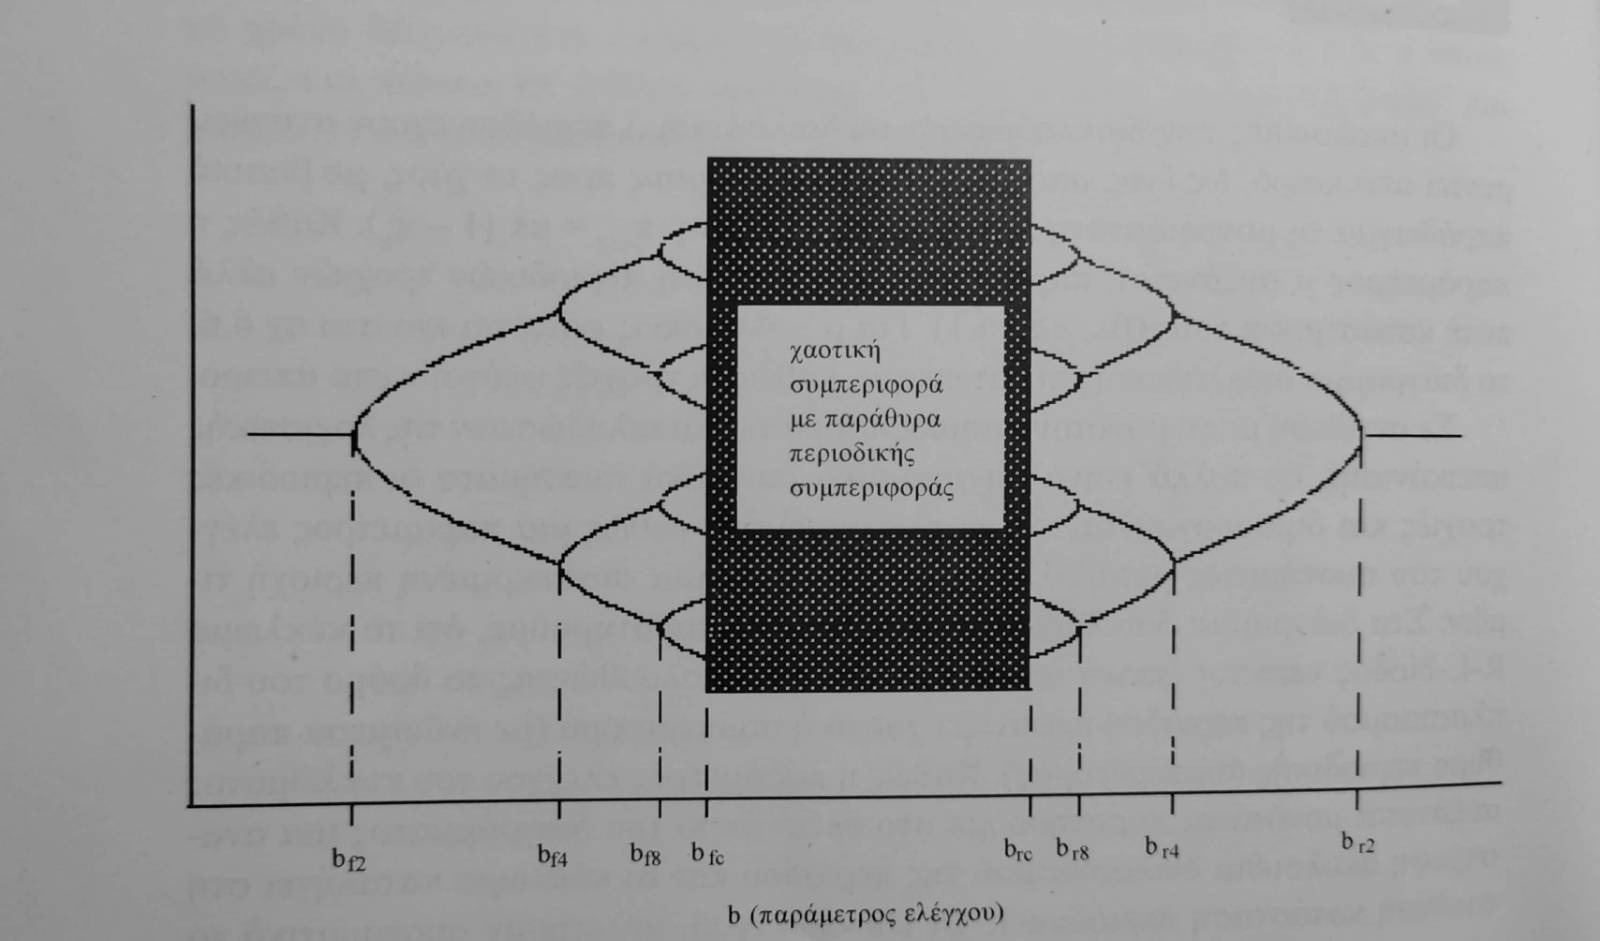
\includegraphics[width=1\linewidth]{LateX images/antimon1}
	\caption{ Σχηματικό διάγραμμα φυσαλίδας περιόδου-1.}
	\label{th:g3}	
\end{figure}

\begin{figure}[ht]
	\centering
	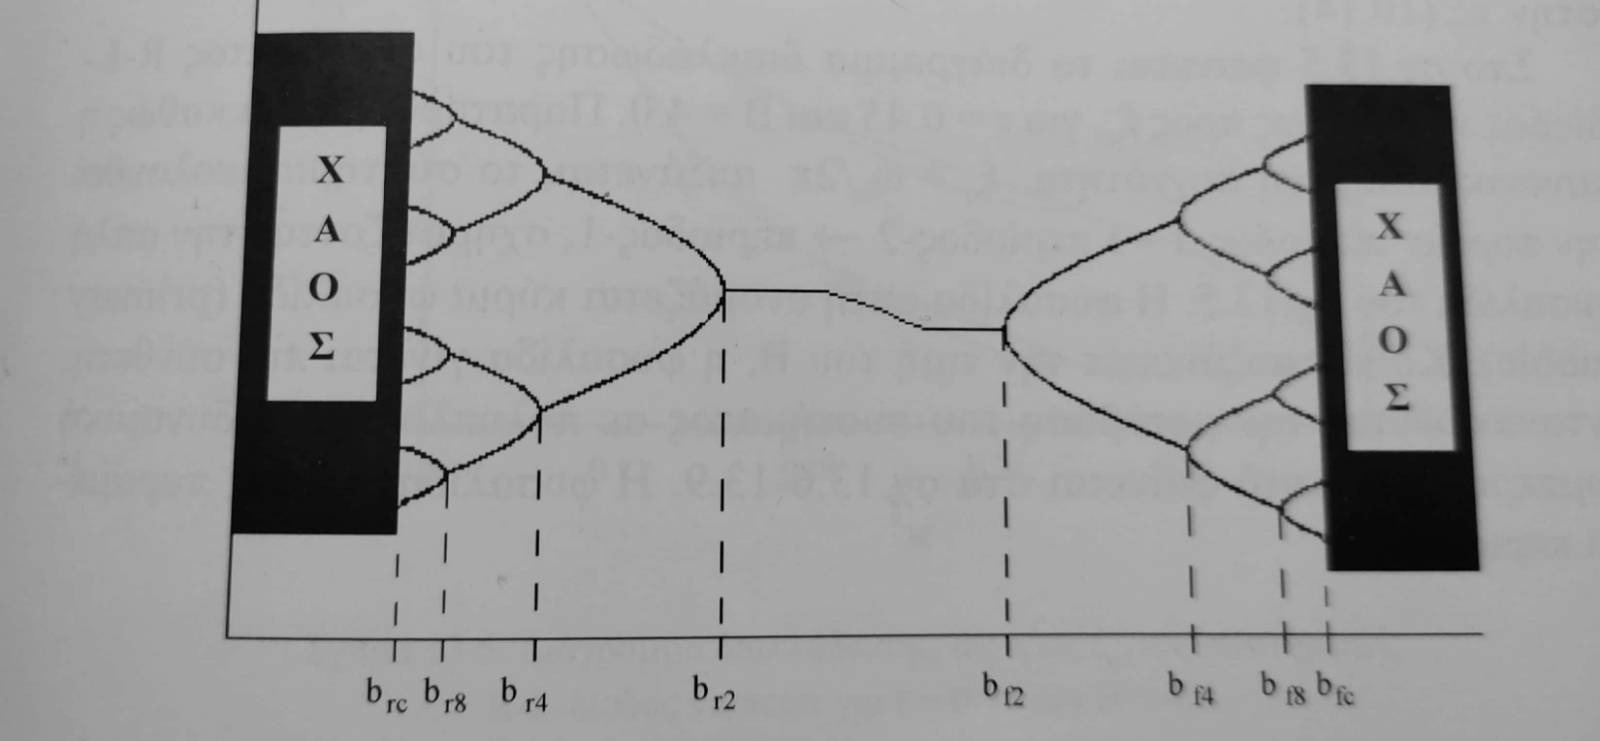
\includegraphics[width=1\linewidth]{LateX images/antimon2}
	\caption{ Σχηματικό διάγραμμα ανάστροφης φυσαλίδας περιόδου-1.}
	\label{th:g4}	
\end{figure}
\subsection{Συνύπαρξη ελκυστών}
Το φαινόμενο της συνύπαρξης ελκυστών είναι το φαινόμενο κατά το οποίο το σύστημα για διαφορετικές αρχικές συνθήκες παρουσιάζει εντελώς διαφορετική δυναμική συμπεριφορά.

\clearpage
